  %%%%%%%%%%%%%%%%%%%%%%%%%%%%%%%%%%%%%%% -*- coding: utf-8; mode: latex -*- %%
  %
%%%%%                        CHAPTER
 %%%
  %

% $Id: 1120-facere-possimus.tex,v 1.1 2007/11/23 09:52:40 david Exp $
% $Log: 1120-facere-possimus.tex,v $
% Revision 1.1  2007/11/23 09:52:40  david
% *** empty log message ***
%
%

  %%%%%%%%%%%%%%%%%%%%%%%%%%%%%%%%%%%%%%%%%%%%%%%%%%%%%%%%%%%%%%%%%%%%%%%%%%%%%
  %
%%%%%                            HEAD MATTER
 %%%
  %

\chapter{Background and Related Work}
%\addcontentsline{lof}{chapter}{\thechapter\quad Facere Possimus}
%\addcontentsline{lot}{chapter}{\thechapter\quad Facere Possimus}
\label{ch:Background}

%\begin{quotation}
%  {\small\it Neque porro quisquam est qui dolorem ipsum quia dolor sit amet, consectetur, adipisci velit...}
%
%{\small\it -- Cerico}
%\end{quotation}




  %%%%%%%%%%%%%%%%%%%%%%%%%%%%%%%%%%%%%%%%%%%%%%%%%%%%%%%%%%%%%%%%%%%%%%%%%%%%%
  %
%%%%%                        FIRST SECTION
 %%%
  %

\section{Distributed File Systems}

Distributed File system is the fundamental storage layer in big data era. They provide a high available storage service with fault tolerance for data corruption, which enable petabytes of data to be persisted across multiple low cost commodity machines reliably.

\subsection{The Google File System}

\subsubsection{Design Principle}
\textit{The Google File System} (GFS) is a scalable distributed file system developed and widely used in \textit{Google Incorporation} for large distributed data-intensive applications. With fault tolerance, it runs on clusters of inexpensive commodity hardware, which provides a storage layer for a large number of applications with high aggregate performance~\cite{ghemawat2003google}. There are some design assumptions for the implementation of GFS:

\begin{itemize}[noitemsep]
	\item The system runs on top on inexpensive commodity hardware so component may often fails.
	\item Files stored on the system are fairly huge than the transitional standards, which means that Gigabyte files are common.
	\item There are three kinds of workloads in the system: large streaming reads, small random reads and large sequential writes which append data to files.
	\item Well-defined semantics for concurrent appends to the same file is needed.
	\item Data processing in bulk with high sustained bandwidth is more important than individual low latency read or write.
\end{itemize}

\subsubsection{The Architecture of GFS}
\noindent The architecture of a GFS cluster consists of a single \textit{master}, multiple \textit{chunkservers}, and is accessed by multiple \textit{clients} as shown in Figure~\ref{fig:gfs}.

\begin{figure}[h]
	\centering
	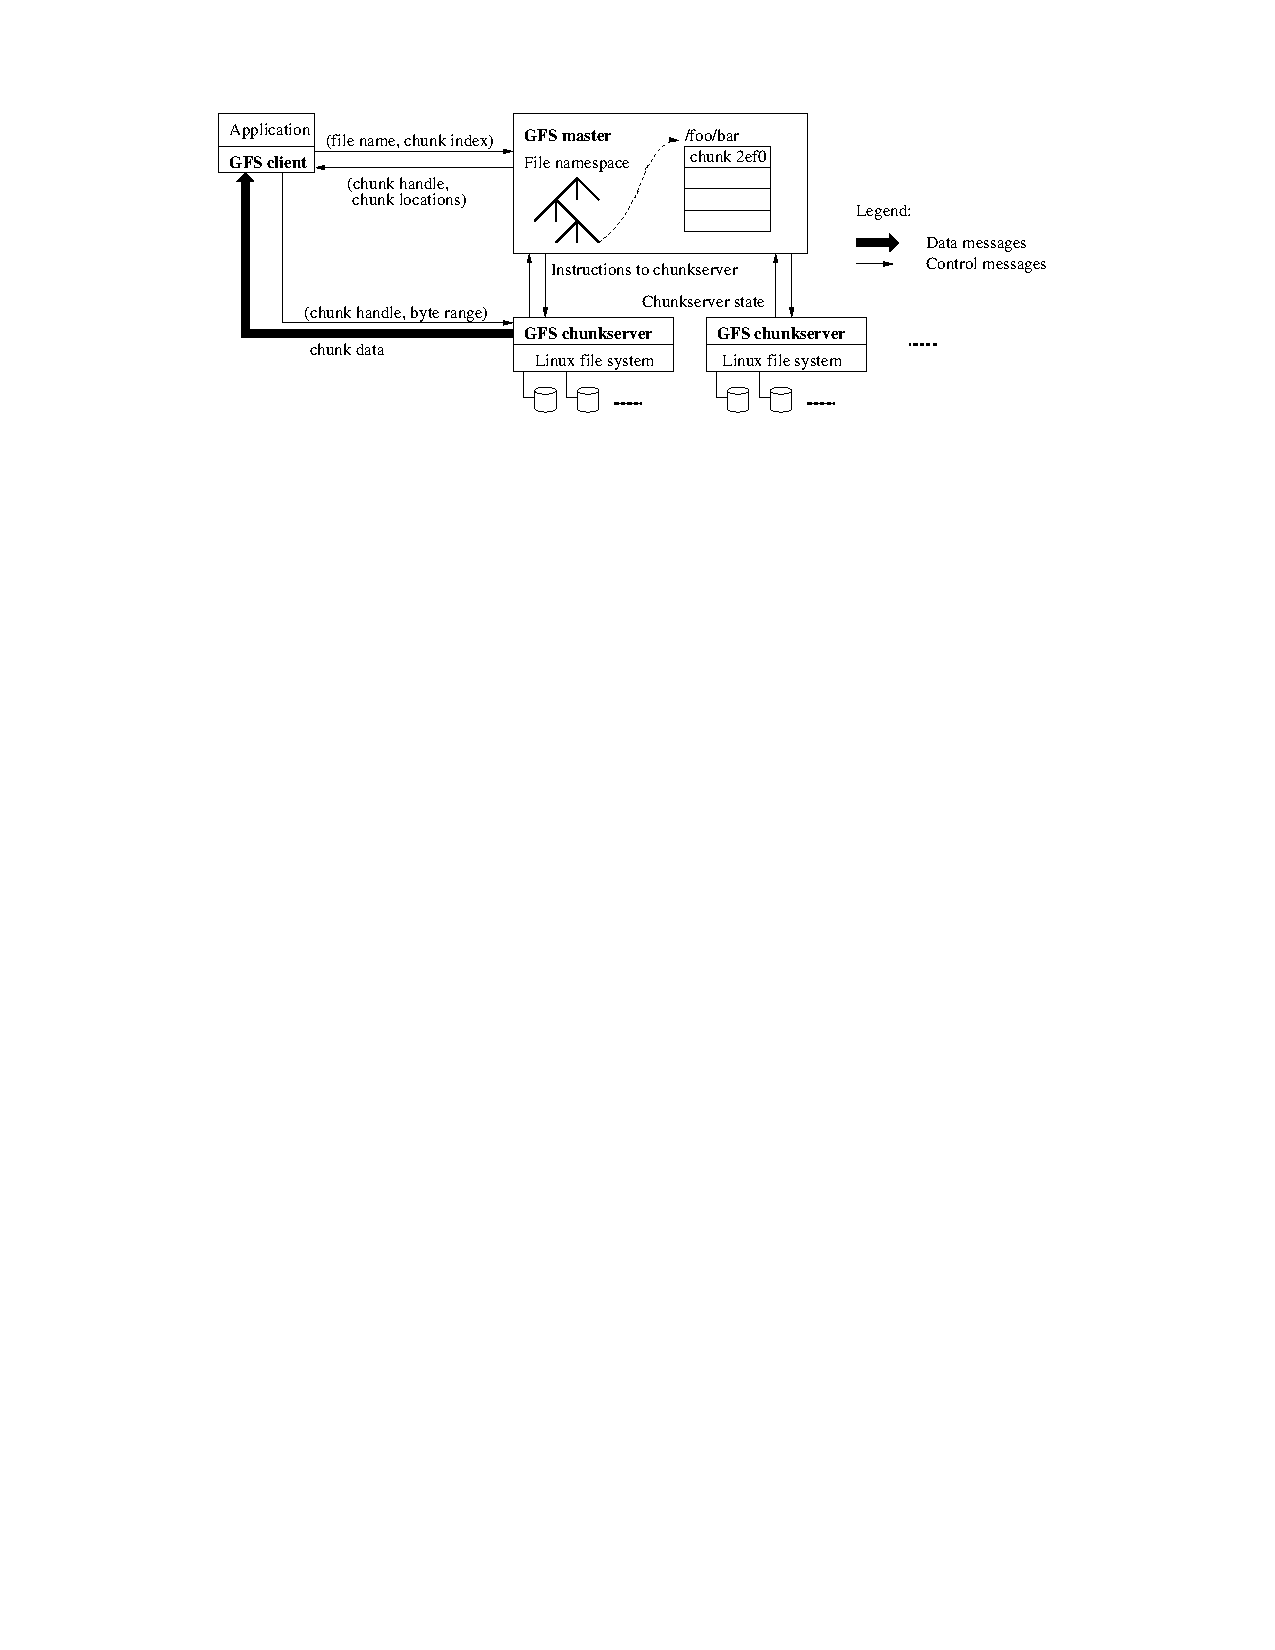
\includegraphics[width=\linewidth]{figs/GFSArchitecture.pdf}
	\caption{The Architecture of GFS \protect \cite{ghemawat2003google}}
	\label{fig:gfs}
\end{figure}

\noindent Files are divided into fixed size \textit{chunks} stored in \textit{chunkservers}. For fault tolerance, each chunk is replicated across multiple chunkservers and the default replication factor is three.

\noindent The \textit{master} is a metadata server maintaining namespace, access control information, the file-chunk mappings and chunks' current locations. Besides, it is also responsible for system-wide activities including garbage collection, chunk lease management and chunk migrations.

\noindent Although this single master server architecture simplifies the design of GFS, especially on complexed tasks like chunk placement and replication decisions using global knowledge, yet the master's involvement in reads and writes needs to be minimized otherwise it will become a bottleneck in the system.

\subsection{The Hadoop Distributed File System}

\subsubsection{Design Principle}
The \textit{Hadoop Distributed File System} (HDFS) is inspired by the Google File System. Initially, HDFS is built for Hadoop Map-Reduce computational framework. With the development of Hadoop ecosystem including HBase~\cite{apachehbase}, Pig~\cite{apachepig}, Mahout~\cite{apachemahout}, Spark~\cite{apachespark}, etc, HDFS becomes the storage layer for all these big data applications. While enabling petabytes of data to be persisted on clusters of commodity hardware at relatively low cost, HDFS aims to stream these large data sets at high bandwidth to user applications. Therefore, like GFS, HDFS is optimized for delivering a high throughput of data at the expense of latency~\cite{white2012hadoop}.

\subsubsection{The Architecture of HDFS}
\noindent Similar to GFS, HDFS stores metadata and file data separately. The architecture of a HDFS cluster consists of a single \textit{NameNode}, multiple \textit{DataNodes}, and is accessed by multiple \textit{clients} as shown in Figure~\ref{fig:hdfsv1}.

\begin{figure}[ht]
	\centering
	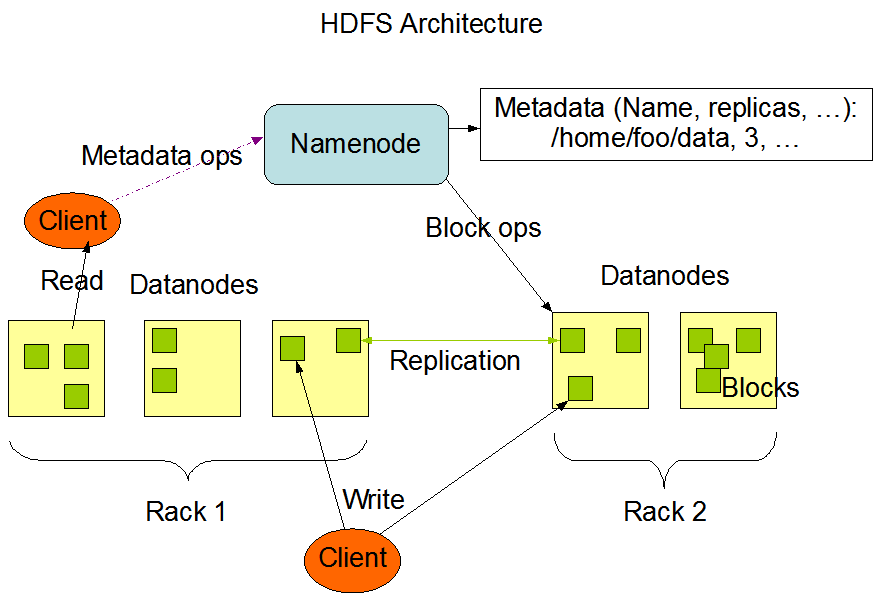
\includegraphics[scale=0.4]{figs/hdfsarchitecturev1.png}
	\caption{The Architecture of HDFS \protect \cite{borthakur2008hdfs}}
	\label{fig:hdfsv1}
\end{figure}

\noindent Files in HDFS are split into smaller blocks stored in \textit{DataNodes}. For fault tolerance, each block is replicated across multiple \textit{DataNodes}.

\noindent The \textit{NameNode} is a single dedicated metadata server maintaining the namespace, access control information, and file blocks mappings to DataNodes. The entire namespace is kept in-memory, called the \textit{image}, of the \textit{NameNode}. Its related persistent record, called the \textit{checkpoint} is stored in the local physical file system. The modification, \textit{editlogs}, of the \textit{image}, called the \textit{journal}, is also persisted in the local physical file system. Copies of the \textit{checkpoints} and the \textit{journals} can made at other servers for durability. Therefore, the \textit{NameNode} restores the namespace by loading the checkpoint and replaying the journal during its restart.

\subsubsection{Single-Writer, Multiple-reader Model}
Once a file is created, written with data and closed by the client application, the bytes written can not be modified. The file can only be reopened for append.

\noindent HDFS implements a \textit{single-Writer, multiple-reader} model using lease management. A HDFS client opens a file for writing is granted a lease for the file and no other client can write to that file at the same time. The writing client needs to renew the lease periodically with the NameNode so that it can keep writing to the file. Otherwise, once the \textit{soft limit} expires, other clients can preempt the lease. If the \textit{hard limit} (one hour) expires and the client didn't renew the lease, HDFS will close the file on behalf of the writer and recover the lease.

\noindent HDFS allows a client to read a file which is open for writing, which means that the lease does not prevent other clients' reading. A file can have multiple concurrent readers.

\section{Concurrency Control and Isolation Level}

\subsection{Concurrency Control in Database Management System}
In a multiuser database management system, \textit{Concurrency Control} permits concurrent users to access a database while preserving the illusion that each user is executing along on a dedicated system~\cite{bernstein1981concurrency}. The main idea is to ensure individual users see consistent states of the database even though users' operations may be interleaved in the shared data.

\noindent In general, there are three concurrency control methods~\cite{franklin1997concurrency}:
\begin{enumerate}[noitemsep]
	\item \textbf{Pessimistic Concurrency Control} (PCC): depends on \textit{Two-Phase Locking} (2PL) to block transactions when running on to the shared data so that interference does not occur.
	\item \textbf{Optimistic Concurrency Control} (OCC): depends on validation to ensure serializability so that before transactions commit, the reads and writes performed by a validating transaction di not conflict with other concurrent transactions. If not, the validating transaction will be aborted and restarted.
	\item \textbf{Multi Version Concurrency Control} (MVCC): when data items are updating by transactions, their previous versions will retain so that other read-only transactions will be provided with these older versions, allowing a consistent snapshot of the database to be presented.
\end{enumerate}

\subsection{Isolation Level for Concurrent Transactions}

\noindent Complete isolation of concurrent running transactions might make one transaction not possible to perform an update into a database table being queried by another transaction. Therefore, real-world databases will provide different levels of transaction isolation so that data consistency will be compromised for performance.

\noindent Four isolation levels are defined in ANSI/ISO SQL-92 specifications~\cite{ansi1992x3}: (1) \textit{Read Uncommitted} (2) \textit{Read Committed} (3) \textit{Repeatable Read} (4) \textit{Serializable}. But a new isolation level, \textit{Snapshot Isolation} and the \textit{anomalies} characterized by isolation types is re-defined in the paper \textit{A Critique of ANSI SQL Isolation Levels}~\cite{berenson1995critique}.

\begin{table}[h]
	\centering
	\begin{tabular}{|c|p{0.8cm}|p{0.8cm}|p{1.5cm}|p{1cm}|p{1cm}|p{1.8cm}|p{1cm}|p{1cm}|}
		\hline
		\textbf{Isolation Level} & \textbf{Dirty Write} & \textbf{Dirty Read} & \textbf{Cursor Lost Update} & \textbf{Lost Update} & \textbf{Fuzzy Read} & \textbf{Phantom} & \textbf{Read Skew} & \textbf{Write Skew} \\ \hline
		Read Uncommitted         & X                    & \checkmark          & \checkmark                  & \checkmark           & \checkmark          & \checkmark       & \checkmark         & \checkmark          \\ \hline
		Read Committed           & X                    & X                   & \checkmark                  & \checkmark           & \checkmark          & \checkmark       & \checkmark         & \checkmark          \\ \hline
		Cursor Stability         & X                    & X                   & X                           & some- times            & some- times           & \checkmark       & \checkmark         & some- times           \\ \hline
		Repeatable Read          & X                    & X                   & X                           & X                    & X                   & \checkmark       & X                  & X                   \\ \hline
		Snapshot                 & X                    & X                   & X                           & X                    & X                   & sometimes        & X                  & \checkmark          \\ \hline
		Serializable             & X                    & X                   & X                           & X                    & X                   & X                & X                  & X                   \\ \hline
	\end{tabular}
	\caption{Isolation Types Characterized by Possible Anomalies Allowed \protect \cite{berenson1995critique}}
	\label{table:anomaly}
\end{table}

\noindent Full definitions of all the anomalies mentioned in Table~\ref{table:anomaly} can be found in the paper \textit{A Critique of ANSI SQL Isolation Levels}. We will discuss how we preclude \textit{fuzzy read, phantom and write skew} in our solution based on \textit{Snapshot Isolation} level in Chapter~\ref{ch:Design}.
\section{MySQL Cluster}

\subsection{Design Principle}
\textit{MySQL Cluster} is a highly available version of MySQL, an open source database management system, with high-redundancy adapted for the distributed computing environment. It integrates the standard MySQL server with an in-memory clustered storage engine called \textit{NDB} (which stands for “Network DataBase”). MySQL Cluster is designed not to have any single point of failure a shared-nothing system running on inexpensive hardware~\cite{mysqlcluster}.

\subsection{The Architecture of MySQL Cluster}
\noindent A MySQL Cluster consists of different processes, called the \textit{nodes}. The communication between the nodes can be seen from Figure~\ref{fig:mysqlclusterarchitecture}. \textit{MySQL Servers} (mysqld, for query processing and NDB data accessing) are the main nodes. \textit{Data Nodes} (ndbd) serve as storage nodes. Besides, there will be one or more \textit{NDB Management Servers} (ndb\_mgmd).

\begin{figure}[h!]
	\centering
	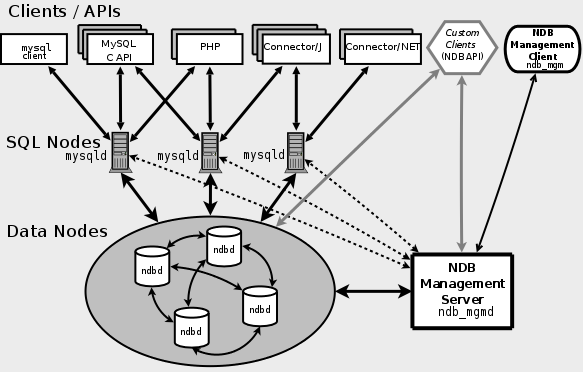
\includegraphics[scale=0.4]{figs/mysqlcluster.png}
	\caption{The Architecture of MySQL Cluster \protect \cite{mysqlcluster}}
	\label{fig:mysqlclusterarchitecture}
\end{figure}

\noindent For fault tolerance, data in MySQL Cluster is replicated across multiple ndbds. Ndbds are divided into \textit{node groups}. Each unit of data is called a \textit{partition} stored by ndbd. The partitions of data are replicated within the same \textit{node group}. The number of \textit{node groups} is calculated as:

\begin{center}
	$Number of Node Groups = \frac{Number of Data Nodes}{Number of Replicas}$
\end{center}

\noindent For example, suppose that we have a cluster consisted with 4 data nodes with replication factor of 2, so there are 2 node groups as shown in Figure~\ref{fig:mysqlclusterng}.

\begin{figure}
	\centering     %%% not \center
	\subfigure[Node Groups in MySQL Cluster]{\label{fig:NGa}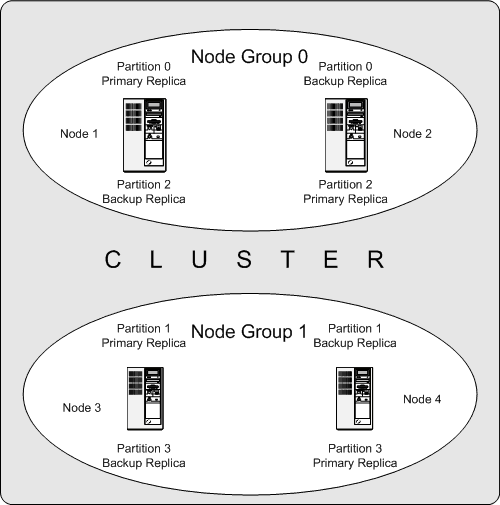
\includegraphics[scale=0.6]{figs/replicas-groups-1-1}}
	\subfigure[Fault Tolerance in Node Groups]{\label{fig:NGb}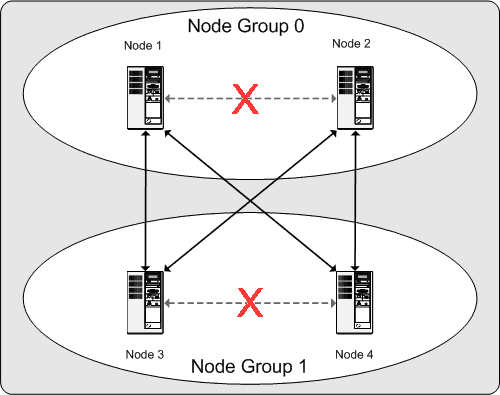
\includegraphics[scale=0.6]{figs/replicas-groups-1-2}}
	\caption{Node Groups in MySQL Cluster and Fault Tolerance \protect  \cite{mysqlclusterng}}
	\label{fig:mysqlclusterng}
\end{figure}

\noindent As we can see from Figure~\ref{fig:NGa}, the data stored in the cluster is divided into four partitions: \textit{0, 1, 2, 3}. Each partition is stored within the same group with multiple replicas. So as long as each participating node group has at least one operating node, the cluster will have a complete copy of the data as shown in Figure~\ref{fig:NGb}. For example, suppose that \textit{Node 2} and\textit{ Node 3} are operating, then partitions \textit{0, 1, 2, 3} remain viable.

\subsection{The Benchmark of MySQL Cluster}
According to the white paper published by Oracle~\cite{mysqlclusterwhitepaper}, MySQL Cluster can handle:
\begin{itemize}[noitemsep]
	\item 4.3 Billion fully consistent reads per minute
	\item 1.2 Billion fully transactional writes per minute
\end{itemize}

\noindent They used an open source benchmarking tool, \textit{FlexAsynch}, to test the performance and scalability of a MySQL Cluster running across 30 commodity Intel Xeon E5-equipped servers, comprised 15 node groups. The result for the write operation performance is shown in Figure~\ref{fig:mysqlwrite}.

\begin{figure}[h!]
	\centering
	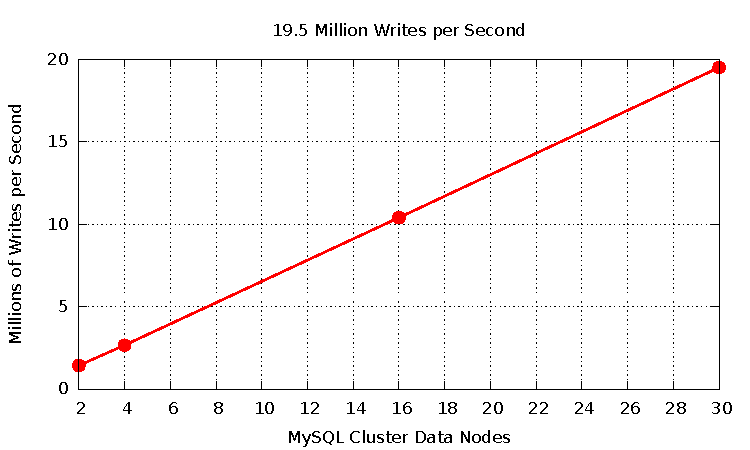
\includegraphics[width=\linewidth]{figs/mysqlclusterbenchmark.pdf}
	\caption{MySQL Cluster Scaling-out Writes Operations}
	\label{fig:mysqlwrite}
\end{figure}

\noindent Therefore, the high operations throughput, \textit{72 million reads and 19.5 million writes operations per second}, of MySQL Cluster makes it the choice to be the distributed in-memory storage layer for the metadata in Hop-HDFS. But the trade off is that the NDB cluster storage engine supports only the \textit{READ COMMITTED} transaction isolation level~\cite{mysqlreadcommited}, which means that we need to put extra effort on the application layer to preclude anomalies in our implementation. See Chapter~\ref{ch:Design}.

\section{Hadoop Open Platform-as-a-service and Hop-HDFS}
\label{sc:Hop-HDFS}
\subsection{Hadoop Open Platform-as-a-service Design Purpose}
The \textit{Hadoop Open Platform-as-a-service} (Hop) ~\cite{hop} is an open platform-as-a-Service (PaaS) support of the Hadoop ecosystem on existing cloud platforms including Amazon Web Service and OpenStack. The goal is to automate the installation of both HDFS and Apache YARN so that unsophisticated users can deploy the stack on the cloud easily by a few clicks from our portal website. 

\subsection{Overcoming Limitations in HDFS NameNode Architecture}

\noindent The storage layer of Hop, called the Hop-HDFS, is a new high available model for HDFS's metadata, aiming to overcome the major limitations of HDFS NameNode architecture:

\begin{itemize}[noitemsep]
	\item \textbf{The scalability of the namespace}: the memory size restricts the storage capacity in the system.
	\item \textbf{The throughput problem}: the throughput of the metadata operations is bounded by the ability of the single machine (NameNode)
	\item \textbf{The failure recovery}: it takes a long time for the NameNode to restart since it needs to load the checkpoint and replay the edit logs into the memory
\end{itemize}

\subsection{The Architecture of Hop-HDFS}

\noindent The architecture of Hop-HDFS consists of multiple \textit{NameNodes}, multiple \textit{DataNodes}, a \textit{MySQL cluster} and is accessed by multiple \textit{clients} as shown in Figure~\ref{fig:hophdfsarchitecture}.

\begin{figure}[h!]
	\centering
	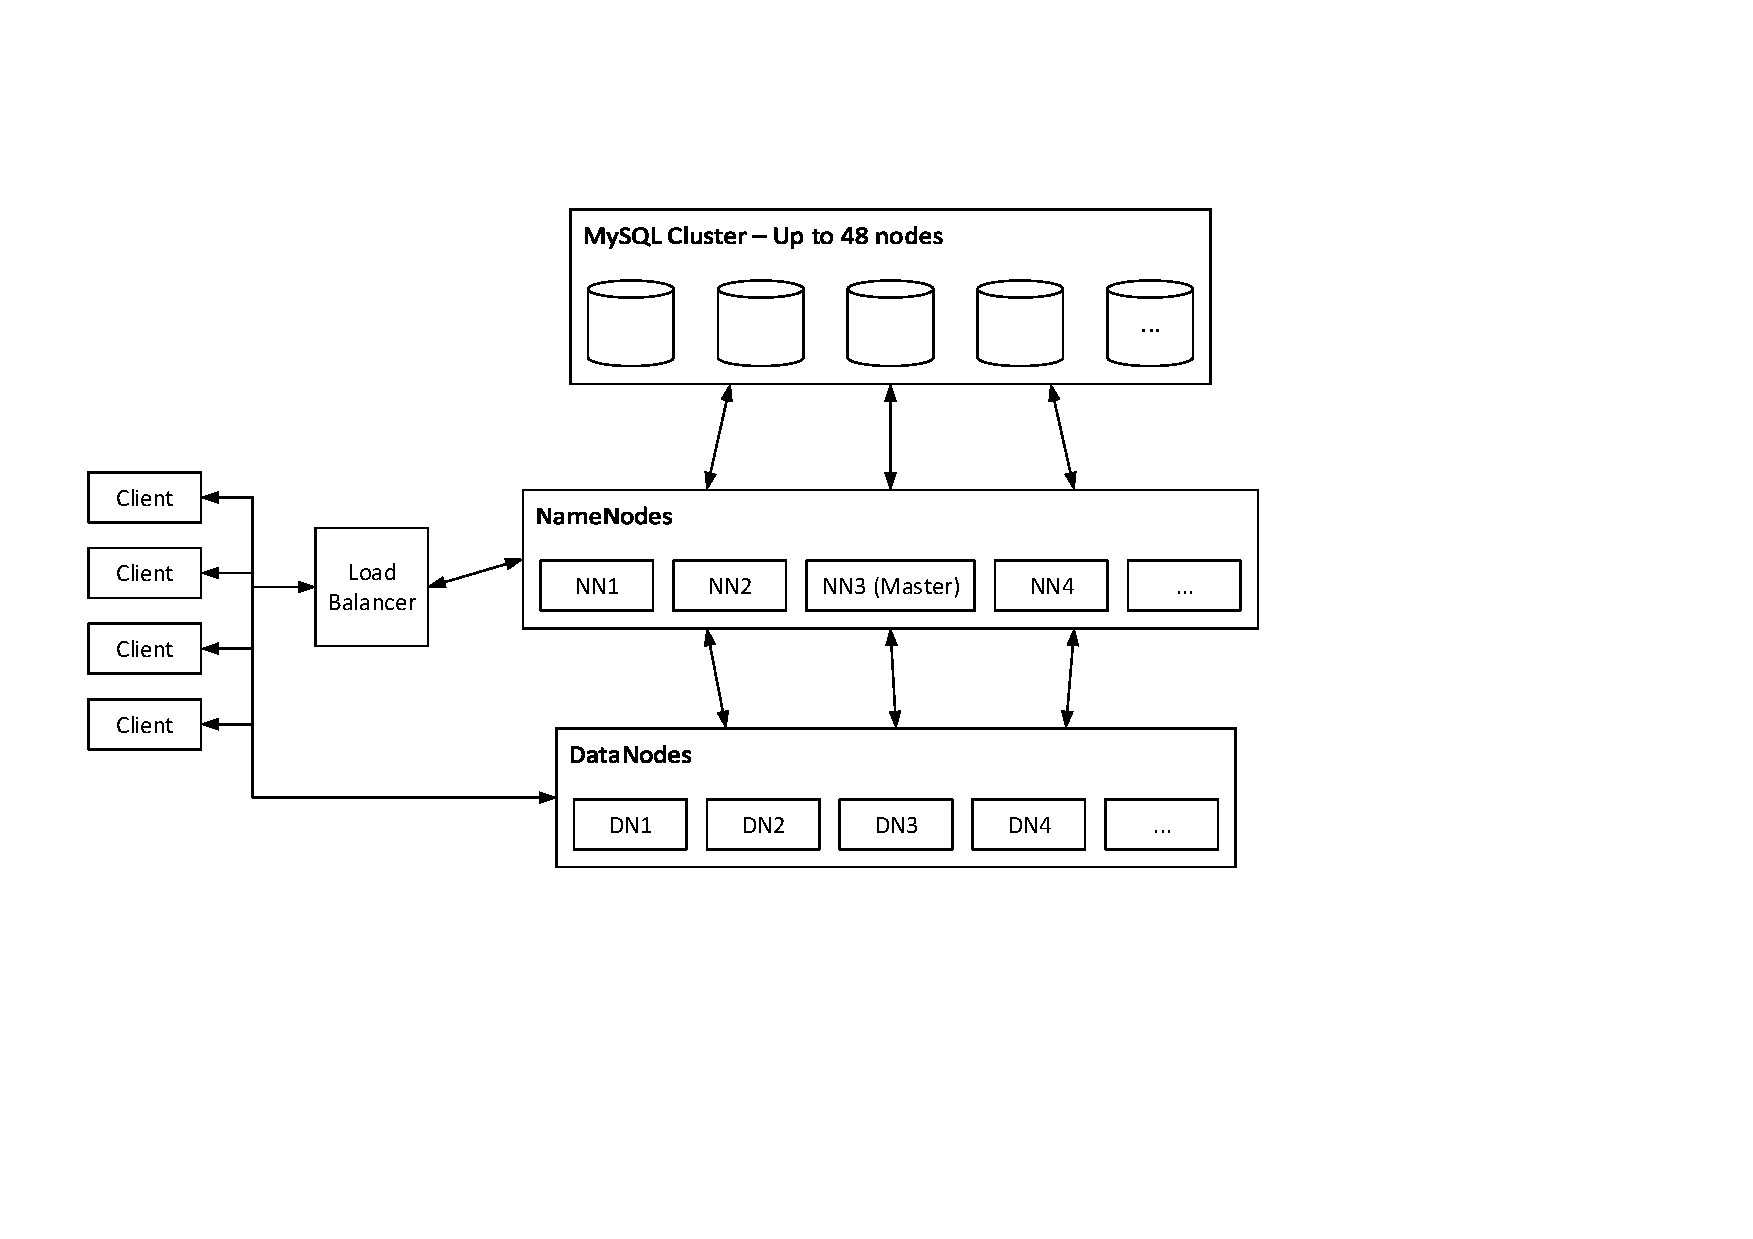
\includegraphics[scale=0.7]{figs/HopHDFSArchitecture.pdf}
	\caption{The Architecture of Hop-HDFS}
	\label{fig:hophdfsarchitecture}
\end{figure}

\noindent The design purpose for Hop-HDFS is to migrate the metadata from NameNode to an external distributed, in-memory, replicated database \textit{MySQL Cluster}. Therefore, the size of the metadata is not limited by a single NameNode's heap size and the scalability problem is solved. We can now have multiple stateless NameNodes architecture so that multiple-writers-multiple-readers are allowed to operate on the namespace to improve the throughput. 

\noindent Moreover, the fault tolerance of the metadata is handled by MySQL Cluster, which grantees high availability of 99.999\%. The \textit{checkpoint} and the \textit{journal} for namespace is not needed, which save time from writing edit logs as well as restarting new NameNodes. Note that we have a leader election in this distributed NameNode architecture. The leader, \textit{master}, will be responsible for tasks like block reporting and statistic functions.

\noindent As we discuss earlier, the size of the metadata for a single file object having two blocks (replicated three times by default) is 600 bytes. It requires 60 GB of RAM to store 100 million files in HDFS, 100 million files is also the maximum storage capacity for HDFS in practice. For MySQL Cluster, it supports up to 48 datanodes~\cite{mysql48nodes}, which means that it can scale up to 12 TB in size with 256 GB RAM for each node in size. But conservatively, we assume that Cluster can support up to 3.072 TB for metadata with a replication of 2, which means that Hop-HDFS can store up to 4.1 billion files. A factor of 40 times increase~\cite{hakimzadeh2014scaling}. 


